% ==============================================================================
% Chapter 8: Project Planning
% ==============================================================================
\chapter{Project Planning}
\label{ch:project_planning}

This chapter details the operational planning, weekly activity distribution, milestone timeline, and project management Gantt chart executed during Project Stage-II in the academic year 2026--2027.

\section{Weekly Planning}
\label{sec:weekly_planning}

The Stage-II project execution was scheduled over a structured 16-week development lifecycle. Table~\ref{tab:weekly_planning} outlines the week-by-week technical activities, assigned team responsibilities, and primary deliverables.

\begin{table*}[htbp]
\caption{Detailed 16-Week Stage-II Project Planning Schedule}
\label{tab:weekly_planning}
\centering
\small
\begin{tabularx}{\textwidth}{lp{0.22\textwidth}p{0.38\textwidth}X}
\toprule
\textbf{Week} & \textbf{Phase / Focus Area} & \textbf{Technical Activities Undertaken} & \textbf{Deliverable} \\
\midrule
\textbf{Week 1--2} & Data Ingestion \& Spatial Pipeline & Curation and ingestion of official NMC survey (7,259 vendors, 308 zones); extraction of OpenStreetMap road vectors and POIs. & Cleaned GIS GeoPackages, normalized dataset baselines. \\
\textbf{Week 3--4} & Spatial Typology \& Transforms & Implementation of logarithmic saturation and proximity decay transforms; unsupervised $K$-Means clustering ($K=2, 4$) across 5 random seeds. & Spatial feature manifest, cluster stability benchmarks ($ARI = 1.0$). \\
\textbf{Week 5--6} & MCDA Engine \& AHP Calibration & Development of 6-factor MCDA scoring; integration of leave-group-out Laplace shrinkage ($M=20.0$); AHP pairwise comparison matrix. & Operational MCDA module, AHP policy validation ($CR \le 0.10$). \\
\textbf{Week 7--8} & Constrained Optimization & Formulation of two-stage pre-emptive Goal Programming (MILP); HiGHS solver integration in \texttt{scipy.milp}; capacity paradox stress-test. & Advisory batch optimizer module, zero-violation proof. \\
\textbf{Week 9--10} & Micro-Slot Packing \& Validation & Development of UTM Zone 43N geometric slot generator; validation on Lekha Nagar pilot site (NN\_F\_013) across Boundaries A and B. & Geometric validation report ($1.87\times 10^{-9}\text{ m}$ edge precision). \\
\textbf{Week 11--12} & Backend Core \& Privacy Security & FastAPI router modularization; SQLite WAL schema setup; HMAC-SHA256 identity hashing; direct Meta WhatsApp Cloud API webhooks. & Production-ready ASGI backend, verified authentication service. \\
\textbf{Week 13--14} & Frontend Portal \& Navigation & React 18 UI development; Leaflet interactive GIS mapping; bilingual (En/Mr) i18n support; in-app walking GPS navigation hook. & Responsive admin console, vendor portal, navigation UI. \\
\textbf{Week 15--16} & Evaluation \& Documentation & 224-scenario MCDA sensitivity audit; automated test suite execution; research paper submission; final Stage-II LaTeX report. & Verified test suite, conference paper, final project report. \\
\bottomrule
\end{tabularx}
\end{table*}

\section{Project Timeline}
\label{sec:project_timeline}

The project roadmap was structured across five major milestone phases:

\begin{enumerate}
    \item \textbf{Milestone 1: Geospatial Ingestion and Baseline Typology (End of Week 4)}
    \begin{itemize}
        \item Ingestion of 7,259 vendor records and 308 municipal zones.
        \item Generation of 12 spatial indicators with logarithmic saturation.
        \item Validation of $K$-Means environmental clusters ($ARI = 1.0$).
    \end{itemize}
    
    \item \textbf{Milestone 2: Multi-Criteria Decision and Optimization Engine (End of Week 8)}
    \begin{itemize}
        \item Deployment of operational 6-factor MCDA with empirical Bayes category shrinkage.
        \item Interactive AHP weight calibration panel with automated $CR \le 0.10$ checking.
        \item Two-stage HiGHS Goal Programming solver resolving the Spatial Capacity Paradox.
    \end{itemize}
    
    \item \textbf{Milestone 3: Metric Micro-Slot Demarcation and Validation (End of Week 10)}
    \begin{itemize}
        \item Reprojection to EPSG:32643 (UTM Zone 43N) eliminating metric distortion.
        \item Packing 10 standardized $2\,\text{m} \times 2\,\text{m}$ slots in the Lekha Nagar pilot.
        \item Verification of $\ge 0.5\,\text{m}$ slot spacing and $1.2\,\text{m}$ continuous pedestrian corridor.
    \end{itemize}
    
    \item \textbf{Milestone 4: Full-Stack Platform, Security, and Multichannel Access (End of Week 14)}
    \begin{itemize}
        \item End-to-end HMAC-SHA256 vendor identity hashing eliminating plaintext phone numbers.
        \item Role-aware React 18 administrative and vendor web portals.
        \item In-app walking navigation with GPS geolocation watching.
        \item Direct Meta WhatsApp Cloud API webhook integration with conversational state machine.
    \end{itemize}
    
    \item \textbf{Milestone 5: Verification, Audit, and Final Reporting (End of Week 16)}
    \begin{itemize}
        \item Completion of the 224-scenario MCDA sensitivity audit (100\% Top-1 stability).
        \item Regression testing across 18 automated test suites.
        \item Submission of conference research paper.
        \item Compilation of the complete institute-compliant Stage-II Project Report.
    \end{itemize}
\end{enumerate}

\section{Gantt Chart}
\label{sec:gantt_chart}

Fig.~\ref{fig:gantt_chart} presents the project Gantt chart, illustrating task schedules, concurrent work streams, and phase dependencies across the 16-week project execution timeline.

\begin{figure*}[htbp]
\centering
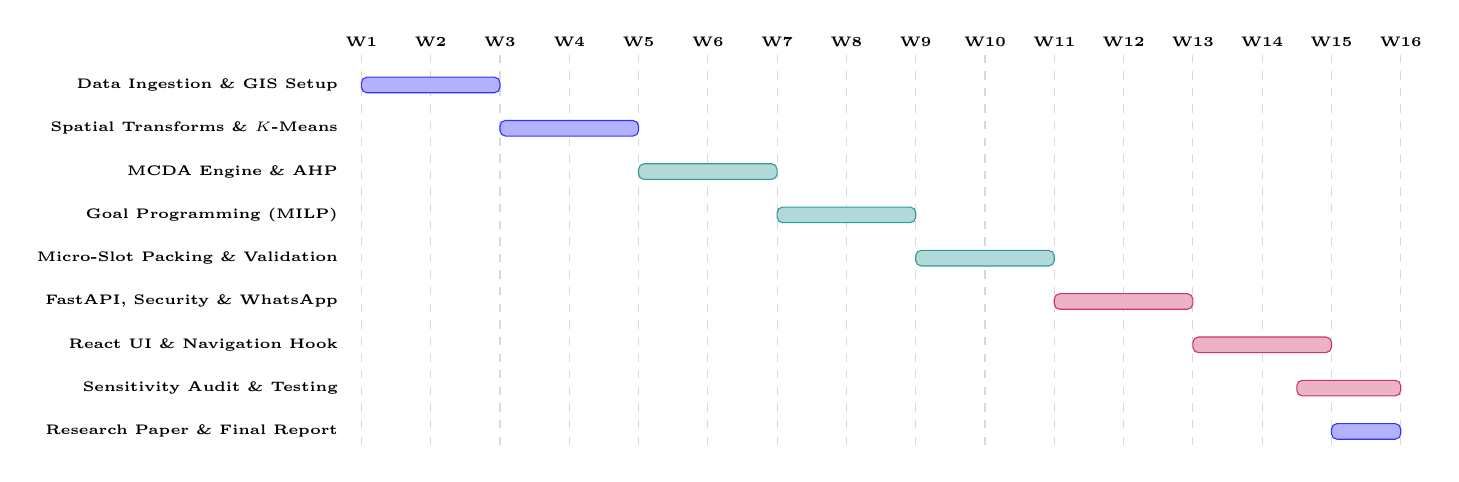
\begin{tikzpicture}[
    x=0.88cm, y=0.55cm,
    font=\tiny,
    taskbar/.style={draw=blue!80, fill=blue!30, rounded corners=2pt, minimum height=0.38cm},
    taskbar2/.style={draw=teal!80, fill=teal!30, rounded corners=2pt, minimum height=0.38cm},
    taskbar3/.style={draw=purple!80, fill=purple!30, rounded corners=2pt, minimum height=0.38cm},
    gridline/.style={dashed, gray!30, line width=0.4pt}
]

% Weeks Header (1 to 16)
\foreach \w in {1,...,16} {
    \node[font=\tiny\bfseries] at (\w, 0) {W\w};
    \draw[gridline] (\w, -0.3) -- (\w, -9.5);
}

% Task Labels & Bars
% Task 1
\node[anchor=east, font=\tiny\bfseries] at (0.8, -1.0) {Data Ingestion \& GIS Setup};
\draw[taskbar] (1, -1.18) rectangle (3.0, -0.82);

% Task 2
\node[anchor=east, font=\tiny\bfseries] at (0.8, -2.0) {Spatial Transforms \& $K$-Means};
\draw[taskbar] (3, -2.18) rectangle (5.0, -1.82);

% Task 3
\node[anchor=east, font=\tiny\bfseries] at (0.8, -3.0) {MCDA Engine \& AHP};
\draw[taskbar2] (5, -3.18) rectangle (7.0, -2.82);

% Task 4
\node[anchor=east, font=\tiny\bfseries] at (0.8, -4.0) {Goal Programming (MILP)};
\draw[taskbar2] (7, -4.18) rectangle (9.0, -3.82);

% Task 5
\node[anchor=east, font=\tiny\bfseries] at (0.8, -5.0) {Micro-Slot Packing \& Validation};
\draw[taskbar2] (9, -5.18) rectangle (11.0, -4.82);

% Task 6
\node[anchor=east, font=\tiny\bfseries] at (0.8, -6.0) {FastAPI, Security \& WhatsApp};
\draw[taskbar3] (11, -6.18) rectangle (13.0, -5.82);

% Task 7
\node[anchor=east, font=\tiny\bfseries] at (0.8, -7.0) {React UI \& Navigation Hook};
\draw[taskbar3] (13, -7.18) rectangle (15.0, -6.82);

% Task 8
\node[anchor=east, font=\tiny\bfseries] at (0.8, -8.0) {Sensitivity Audit \& Testing};
\draw[taskbar3] (14.5, -8.18) rectangle (16.0, -7.82);

% Task 9
\node[anchor=east, font=\tiny\bfseries] at (0.8, -9.0) {Research Paper \& Final Report};
\draw[taskbar] (15, -9.18) rectangle (16.0, -8.82);

\end{tikzpicture}
\caption{Gantt chart illustrating the 16-week project execution timeline and task dependencies.}
\label{fig:gantt_chart}
\end{figure*}
